%%%%%%%%%%%%%%%%%%%%%%%%%%%%%%%%%%%%%%%%%%%%%%%%%%%%%%%%%%%%%%%%%%%%%%%%%%%%%%%%
%2345678901234567890123456789012345678901234567890123456789012345678901234567890
%        1         2         3         4         5         6         7         8
\documentclass[conference]{IEEEtran}
%\documentclass[letterpaper, 10pt, conference]{ieeeconf}  % Comment this line out if you need a4paper
%\documentclass[a4paper, 10pt, conference]{ieeeconf}      % Use this line for a4 paper
%\IEEEoverridecommandlockouts                              % This command is only needed if you want to use the \thanks command
%\overrideIEEEmargins
% See the \addtolength command later in the file to balance the column lengths
% on the last page of the document
% The following packages can be found on http:\\www.ctan.org
\usepackage{graphics} % for pdf, bitmapped graphics files
\usepackage{epsfig} % for postscript graphics files
\usepackage{mathptmx} % assumes new font selection scheme installed
\usepackage{times} % assumes new font selection scheme installed
\usepackage{amsmath} % assumes amsmath package installed
\usepackage{amssymb}  % assumes amsmath package installed


%\usepackage{enumitem}
%\usepackage{amsfonts
\usepackage{booktabs}
\usepackage{tikz}
\usetikzlibrary{automata, positioning}

%%%%%%%%%%%%%%%%%%%%%%%%%%%%%%%%%%%%%%%%%%%%%%%%%%%%%%%%%%%%%%%%%%%%%%%%%%%%%%%%%%%%

\title{\LARGE \bf Visualization and Quantification of Supply Chain Risks for Global Retailers and Manufacturers}

%\author{ \parbox{3 in}{\centering Dieudonne N. Ouedraogo*
%         \thanks{*Use the $\backslash$thanks command to put information here}\\
%         Faculty of Electrical Engineering, Mathematics and Computer Science\\
%         University of Twente\\
%         7500 AE Enschede, The Netherlands\\
%         {\tt\small h.kwakernaak@autsubmit.com}}
%         \hspace*{ 0.5 in}
%         \parbox{3 in}{ \centering Pradeep Misra**
%         \thanks{**The footnote marks may be inserted manually}\\
%        Department of Electrical Engineering \\
%         Wright State University\\
%         Dayton, OH 45435, USA\\
%         {\tt\small pmisra@cs.wright.edu}}}

\author{
	Dieudonne N. Ouedraogo\\
	\texttt{douedra1@binghamton.edu}
	\and
	Hayford K. D. Adjavor\\
	\texttt{hadjavo1@binghamton.edu}
		\and
	Saraswathi Hathikal\\
	\texttt{shathik1@binghamton.edu}
		\and
	 Aishwarya Shivachandar\\
	\texttt{faishwa1@binghamton.edu}
		\and
	Nagendra N. Nagarur*\\
	\texttt{nnagarur@binghamton.edu} \thanks{Nagendra N. Nagarur is with Faculty of Industrial Systems Engineering, Department of Systems Science and Industrial Engineering, Thomas Watson School of Engineering and Applied Sciences, State University of New York at Binghamton, 4400 Vestal Pkwy E., Vestal, NY 13905.{\tt\small nnagarur@binghamton.edu}}} % <-this % stops a space}

%%%%---------------This another version of the author list below ---------------%%%
%%\author{Dieudonne N. Ouedraogo$^{1}$, Hayford K. D. Adjavor$^{2}$,Saraswathi Hathikal$^3$, Aishwarya Shivachandar$^4$, and Nagendra N. Nagarur$^5$ % <-this % stops a space
%	\thanks{*This work was not supported by any organization}% <-this % stops a space
%	\thanks{$^{1}$H. Kwakernaak is with Faculty of Electrical Engineering, Mathematics and Computer Science,
%		University of Twente, 7500 AE Enschede, The Netherlands
%		{\tt\small h.kwakernaak at papercept.net}}%
%	\thanks{$^{2}$P. Misra is with the Department of Electrical Engineering, Wright State University,
%		Dayton, OH 45435, USA
%		{\tt\small p.misra at ieee.org}}%
%}

%%%%%%%%%%%%%%%%%%%%%%%%%%%%%%%%%%%%%%%%%%%%%%%%%%%%%%%%%%%%%%%%%%%%%%%%%%%%%%%%%%%%%%%%%%%

\begin{document}

\maketitle
\pagenumbering{arabic}
\thispagestyle{empty}
\pagestyle{empty}


%%%%%%%%%%%%%%%%%%%%%%%%%%%%%%%%%%%%%%%%%%%%%%%%%%%%%%%%%%%%%%%%%%%%%%%%%%%%%%%%
\begin{abstract}

A retailer with global presence must have a healthy, robust supply chain. Towards this end, the retailer must develop a good plan to quantify significant supply chain risks and build appropriate mitigation resources. The goal of this study is to identify, quantify, and visualize potential risks to a global retailer’s supply chain network and recommend better mitigation tools. To achieve this desired outcome, this paper combines network science and operations research methodologies. It builds a simplified decision-making model, where the risk factors of a global supply chain could be perceived as a network with nodes in which the value-at-risk and location are associated with each node. A unique value-at-risk exists at each node in the supply chain. Value-at-risk in our model represents the product of the risk exposure index and the probability of annual loss for the node. A preliminary review of available literature shows good prospects in terms of application to similar problems in this area of research.
\end{abstract}

\begin{IEEEkeywords}
	Global supply chain risk, network science, and OR approach.
\end{IEEEkeywords}
%%%%%%%%%%%%%%%%%%%%%%%%%%%%%%%%%%%%%%%%%%%%%%%%%%%%%%%%%%%%%%%%%%%%%%%%%%%%%%%%
\section{Introduction}

Globalization is extending local supply chain across boundaries to accommodate customers’ demands throughout the world. It has created a connected economic environment unlocking new markets and bringing new customers onboard. It has dramatically changed the business operations opening doors for better opportunities. However, the associated risks are significantly growing with an increased level of globalization. For instance, the number of natural disasters affecting the commerce has only been drastically increasing over the past few decades [1]. These repetitive and large occurrences of natural disasters and huge economic fluctuations disrupt the supply chain operations. Identifying the relevant major risks and addressing them with a suitable mitigation strategy will provide the companies with an added advantage to compete and survive in this ever-growing competitive global market. Supply chains are invariably exposed to a multitude of challenges that prime the companies to expanded their capabilities to mitigate the overall impact. Supply chain managers need to make well-informed decisions to make the best of the opportunities and design strategies to hedge these unexpected uncertainties. Uncertainties and related risks are inevitable in supply chain/web, nevertheless, efficient risk management and readiness to handle the unseen situation is vital to outlive in the growing market. As there is no silver-bullet strategy to shield against all the risks, executives need to make necessary trade-offs to mitigate and prioritize major risks.

\section{Literature Review}
\cite{c4} the study investigates the effect on the equity risk and stock prices due to the supply chain disruption for the period of 1989-2000. Equity risk and stock price further impact the various stakeholders i.e. investors, supplier, employees, management board and mainly the customers. The paper quantifies the economic risk of the firm due to any supply chain disruption and the long-term stock price effect. It justifies that the investments made in increasing responsiveness and reliability of the supply chain to establish a mitigation strategy that improves the real-time visibility, anticipating disruptions and related effects.\newline
\cite{c5}, the paper explores the use of integrated approach in handling supply chain risks such as the use of (r,Q) policy for inventory management and choosing a suitable location for the inventory, using a linear integer programming and algorithm to study the probability of a supply chain disruption etc. The study uses a “Lagranian Relaxation” approach to study the disruption and response probability and quantifies the related economic losses for a dynamically sourced supply chain design to capture and study the impact of risk pooling and risk diversification. It justifies that studying the probability of disruptions and improved preparedness reduces the threat cause by the supply chain disruptions.\newline
\cite{c3}, the paper discusses various methods of building a resilient supply chain to address the vulnerability of supply chain in today’s market by developing proper management and mitigation strategy. The effects of several strategies such as mapping, sourcing decision, efficiency vs. redundancy tradeoff, collaborative planning, creating a supply chain risk management culture in workplaces, creating visibility of the risks etc. is discussed in order to develop a robust action plan.\newline

\cite{c8}, the article explores an initiative to study the risk and vulnerability associated with globalizing supply chain and transport network for the year 2012. As these (globalization and transportation) form the pillar of the global economy today, the impact of the associated risks is devastating resulting in huge financial losses. The article further discusses the results of the workshops conducted in different parts of the world to deepen the problem understanding and identify the risk landscape. Effect of natural disasters, political factors, terrorism, geopolitical restrictions, supply-demand variation etc. is studied and suitable solutions to fight the volatility is analyzed.

\section{Problem Statement}
Global and local supply chains are constantly subjected to numerous risks as they expand geographically and operationally. Certain risks can cause major and irrecoverable disruption to the supply chain and the intensity of disruption depends on the source and nature of the risks. In order to focus on the risks causing catastrophic impact, companies need appropriate tools to identify, quantify and model the risk factors. Even so, quantifying the supply chain risks merely indicate the degree of impact, comprehensive and powerful tool to quantify and visualize the major risks in the different locations is the need of the hour. 

\section{Geographical Scope}
\subsection{Facility Sites/Location}
\ref{RiskLocations} illustrates the locations analyzed in our simulation with associated risks.

\begin{table}[h!]
\centering
\caption{Risk Location List}
\label{RiskLocations}
\begin{tabular}{|p{2cm}||p{2cm}|p{2cm}|}
\hline
\multicolumn{3}{|c|}{Selected Global Risk Locations} \\
\hline
Loc. Name & Loc. Name & Loc. Name \\
\hline
Buenos Aires & Salvador  & Arteixo \\
Paris & Mumbai & Montreal \\
Melbourne & Mexico City & Ankara \\
Saint Petersburg & Tijuana & Monterrey \\
Abidjan & Casablanca & Roma \\
Nairobi & Istanbul  & Porto \\
\hline
\end{tabular}
\end{table}

\section{Types of Risks}
\ref{RiskTypes} shows the various types of the risks sampled for this study.

\begin{table}[h!]
\centering
\caption{Types of Risks}
\label{RiskTypes}
\begin{tabular}{|p{1.5cm}||p{1.5cm}|p{1.5cm}||p{1.5cm}|}
\hline
\multicolumn{4}{|c|}{Selected Types of Risks} \\
\hline
Financial & Harzardous & Strategic & Operational\\
\hline
Credit default & Natural disasters  & New technology &  Suppliers issues \\
Interest rate fluctuations & Wildfire/Tornadoes & New competition & Cyber attack \\
Fuel prices & Missing Cargoes & Change in demand &  Theft of resources \\
Tax laws changes & Building fire & Negative media & Loss of key personnel \\
Economic Recessions & Product liability & Ethic violation & Logistic issues \\
Liquidity/Cash & Facility loss  & Technologies choices & Health/safety violations \\
\hline
\end{tabular}
\end{table}

\section{Impact \& Consequences of Risks}
\ref{ImpactsConseqRisks} shows a summary of this factors.
\begin{figure}[h!]
\centering
\includegraphics[scale=0.5]{fig2.PNG}
\caption{Impacts/Consequences of Risks}
\label{ImpactsConseqRisks}
\end{figure}

\section{Methodology}
\subsection{Mathematical Model and Analysis}
Assuming that the company has manufacturing facilities at locations named Nm (generally, $N_m \leqslant 25$ which include warehouses and distribution centers) and number of stores Ns (for a globally present company, usually $N_s \geqslant 1000$ locations). Hence, the total number of locations is as given below:
$Nm + Ns=N$

\subsubsection{Assumption Underlying Model}
The following are some of the assumptions underlying our mathematical modeling adopted in this study.
	
\begin{itemize}
\item  Aggregate probability of experiencing a loss for the company at any given place in the supply chain is derived from the same distribution or process. The company is less likely to open a location if it is subjected to higher risks (financially or weather wise or any type of associated risks) compared to its current locations.
\item  Global presence is a gradual phenomenon based on extensive research. Hence, company’s historical data is used to estimate the parameters of the distribution or the process that are derived from the supply chain modeling.
\item Time series data from the company are used to record the number of major issues at a particular location and its corresponding impact on the location. Further, the time to recovery and other useful metrics are calculated.
\end{itemize}

\subsubsection{Modeling the Time \& the Type of Events in the Supply Chain Using Markov Chain}
Suffice to mention that the major contribution of this work to the existing literature of the topic is the attempt to model the global supply risk as a Markov Chain are illustrated below.\\\\ Various techniques are available to model the supply chain. In this research, Markov chain modeling is implemented. Consider that the locations open and join the supply chain according to a Poisson process at a rate v (rate is estimated based on the company’s past data). Each location remains joined to the supply chain (without disruption) for a specific amount of time which is exponentially distributed with rate μ and then get disrupted (major disruption). Independently, each location is subjected to an impact due to the issues and other risks according to a Poisson process at a rate of $\lambda$.\\\\ All impact sizes are independent and identically distributed with the same distribution (estimated based on the historical data). Revenue generated at each location is $c$ per unit time. At any given time $‘t’$, the number of locations $N =N_m+N_s$. Let the random variable $X_1$ denote the time until a new location is open, $X_2$ denote the time until the current location experiences a major disruption, and $X_3$ denote the time when there is a negative impact or effect on the entire chain value. Then, by the Poisson/exponential assumptions of memoryless property of the exponential distribution, these 3 random variables are independent and exponentially distributed:\newline
$$
X_1 \sim \operatorname{exp}\left({v}\right)
$$
$$
X_2 \sim \operatorname{exp}\left({N \mu}\right)
$$
$$
X_3 \sim \operatorname{exp}\left({N \lambda}\right)
$$
$X_1$:Time until the next event from the Poisson rate v process.
$X_2$:represents N locations, each independently with their own opening (joining) time " $Y_1,...,Y_N$ exponential at rate μ. Thus $X_2 = min {Y_1,...,Y_N}$, which is exponential at rate $N\mu$ because $P(X_2>x)=P(Y_1>x,...,Y_N>x) = P(Y>x)^N=exp(\neg N\mu x).$
Similar to $X_2$, $X_3 \sim \operatorname{exp}\left({N \lambda}\right)$ as it is the minimum of N iid $exp(\lambda)$. Hence supply chain behavior overtime can be modelled as a Markov chain with 3 types of events as follows:\newline
$S_1$: a new store (location open)
$S_2$: an existing store or locations close (disrupted) as a result of a catastrophic event 
$S_3$: an impact (loss) is recorded (or comes in) on the company value or return.
\\\\
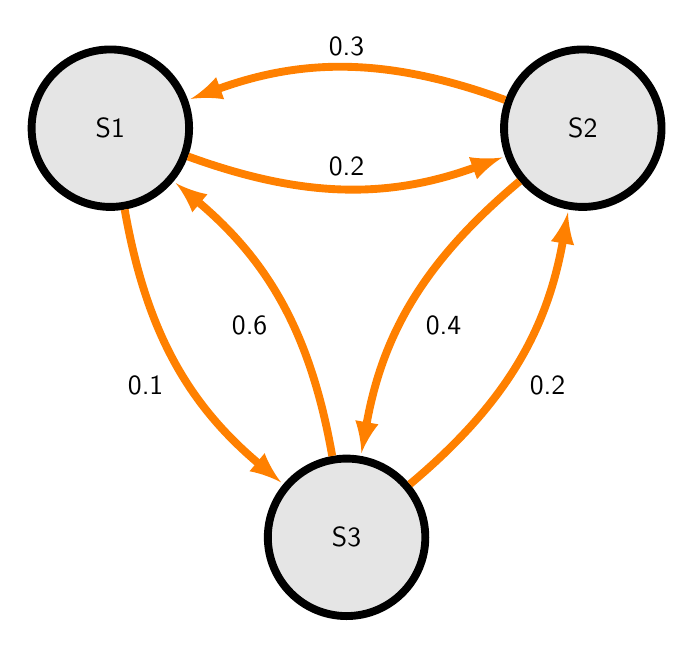
\begin{tikzpicture}[font=\sffamily]
% Setup the style for the states
\tikzset{node style/.style={state, 
		minimum width=2cm,
		line width=1mm,
		fill=gray!20!white}}
% Draw the states
\node[node style] at (0, 0)      (S1)     {S1};
\node[node style] at (6, 0)      (S2)     {S2};
\node[node style] at (3, -5.196) (S3) {S3};

% Connect the states with arrows
\draw[every loop,
auto=right,
line width=1mm,
>=latex,
draw=orange,
fill=orange]
(S1)     edge[bend right=20]            node {0.1} (S3)
(S1)     edge[bend right=20, auto=left] node {0.2} (S2)
(S2)     edge[bend right=20]            node {0.3} (S1)
(S2)     edge[bend right=20, auto=left] node {0.4} (S3)
(S3) edge[bend right=20]            node {0.2} (S2)
(S3) edge[bend right=20, auto=left] node {0.6} (S1);
\end{tikzpicture}

The time until the next event is the minimum m = min ${X_1,X_2,X_3}$, hence is itself exponentially distributed with rate $r=v+N\mu+N\lambda$ which is the sum of the three rates. Thus, if the current time is $‘t’$ and there are N locations, then “next event” can be predicted at time $t+(-(1/r) ln(U), (0<U<1)$ \newline
To determine the type of event: Noting that each of $X_1, X_2$ or $X_3$ will be the minimum with probabilities $p_1=v/r$, $p_2=N\mu/r$, $p_3=N\lambda/r$, independently generate a random variable $C$ with distribution $P(C=1)=p_1$, $P(C=2)=p-2$, $P(C=3)=p_3;$ if $C=i$ it implies that the event is of type $S_i$. We therefore generate $U$.\newline
If $U<=p_1$,then set $C=1$. If $p_1<U<=p_1+p_2$, then set $C = 2$. If $U > p_1+p_2$, then set $C = 3$.

\subsection{Modeling the Total Risk on the Chain Using Aggregate Loss}
Aggregate loss is the total amount of loss in one period. It can be modelled as follows:
\begin{itemize}
\item Individual risk model
\item Collective risk model
\end{itemize}

In individual risk model, aggregate loss is defined by $S = X_1+....+X_n$ where the risks(losses) ${X_1,....,X_n}$ are stochastically independent. The number of locations is denoted as ‘n’ and $X_{i}$ is the impact size for the location ‘i’. There is positive chance that the location ‘i’ will not have any impact in the period of study $P(X_i=0)>0$.\newline 
In collective risk model, aggregate loss is defined by $S=X_1+...+X_N$ where the risks(losses) ${X_1,X_2,...}$ are stochastically independent and identically distributed (i.i.d.) and where N is a discrete random variable (called frequency) indicating the number of risks (losses), and that the $X_i’s$ are independent of N. The number of impacts is denoted as ‘N’ and $X_i$ denotes the i-th amount of the impact that has occurred. The distribution of N is called the primary distribution and the common distribution of $X_i’s$ is called the secondary distribution. This model is a special case of compound distribution in which random number of identically distributed random variables are added. In collective model, $P(X_i=0)=0$, For $N = 0$; $S = 0$.\newline
If $‘M’$ is the total number of incidents on the supply over a defined period $‘T’$, based on the data, the probability of incidences at location $‘i’$ is obtained by the following equation:\newline
\[ p_i
= \frac{\text{total incidence at location 'i'}}{\text{total incidence in the supply chain}}
\]

\section{Results \& Discussion}
\subsection{Simulation}

\begin{table}[h!]
\centering
\caption{Sampled Results from Markov Simulation}
\label{NumericalResult_Markov}
\begin{tabular}{|p{1.5cm}||p{1.5cm}|p{1.5cm}||p{1.5cm}|}
\hline
\multicolumn{4}{|c|}{Numerical Results from Markov Simulation} \\
\hline
Event & Time & Event Type & Probability of Occurrence \\
\hline
Next Event & 0.1191249  & It's a loss being recorded in the chain &  0.2800 \\
** & 0.1289076 & It's a loss being recorded in the chain & 0.2800 \\
** & 0.1360933 & It's a loss being recorded in the chain &  0.2800 \\
** & 0.1415372 & It's location's disruption & 0.7000 \\
** & 0.1429596 & It's location's disruption & 0.6977 \\
** & 0.1575537 & It's a loss being recorded in the chain & 0.1760 \\
** & 0.6944444 & It's a new location joining the chain & 0.1950 \\
\hline
\end{tabular}
\end{table}

\begin{figure}[thpb]
\centering
\includegraphics[scale=0.25]{fig4.PNG}
\caption{Sorted Simulation Values}
\label{SortedValues}
\end{figure}

\subsubsection{Visualization}

\begin{table}[h!]
\centering
\caption{Risk Locations By Category}
\label{RiskLocAndCategory}
\begin{tabular}{|p{2cm}||p{2cm}|p{2cm}|}
\hline
\multicolumn{3}{|c|}{Risks \& Categories} \\
\hline
High Risk Loc. & Medium Risk Loc. & Low Risk Loc. \\
\hline
Buenos Aires & Tijuana  & Ankara \\
Paris & Casablanca & Monterrey \\
Melbourne & Istanbul & Roma \\
Saint Petersburg & Arteixo & Porto \\
Abidjan & Montreal & \\
Nairobi & Istanbul  &  \\
Salvador &  &  \\
Mumbai &  &  \\
Mexico City &  &  \\
\hline
\end{tabular}
\end{table}


\begin{figure}[thpb]
	\centering
	\includegraphics[scale=0.25]{fig7.PNG}
	\caption{Location By Categories}
	\label{LocByCategory}
\end{figure}

\begin{figure}[thpb]
	\centering
	\includegraphics[scale=0.25]{fig6.PNG}
	\caption{Aggregate Risk By Location}
	\label{AggregateRiskLoc}
\end{figure}

\section{Conclusion \& Recommendations}
The results (\ref{SummaryChart}) clearly indicate as to how simulation and visualization can be used as a tool for risk identification and assessment, likelihood of occurrence and impact of the supply chain risks. It is imperative to establish a baseline, analyze the probability and related impact of the risk. For all the leading companies in today’s market adaption of advanced tools such as visualization helps in prioritizing risks by the threat (based on analysis), bolster the supply chain resilience i.e. having a robust mitigation plan in place.\newline

\begin{figure}[thpb]
	\centering
	\includegraphics[scale=0.45]{fig9.PNG}
	\caption{Summary Chart of Risk Identification \& Assessment}
	\label{SummaryChart}
\end{figure}
Supply chain risk mitigation strategy framework begins with use of advanced tools to identify and quantify the risks followed by taking a holistic view of the operating units in the supply chain and ensure the risk factors are accurately prioritized and a strategy is built to overcome these risks.

The major factors involved in the supply chain risk mitigation strategy are shown in \ref{MitigatingFactors}.

\begin{figure}[thpb]
	\centering
	\includegraphics[scale=0.45]{fig10.PNG}
	\caption{Major factors to be considered while developing a supply chain risk mitigation strategy}
	\label{MitigatingFactors}
\end{figure}

\begin{itemize}
\item Framework to mitigate risks
\item It is possible to model and simulate the system with a Markov Process
\item  Visualization is powerful tool in decision-making
\item  Choose financially strong, competent world-class suppliers.
\item  compressing global shipping time and cycle time variation.
\item Track global shipments and take action promptly
\end{itemize}

\section{Future Work}
\begin{itemize}
\item Markov chain analysis could be expanded
\item Parameter estimation of risk and impacts
\item Build an interactive software
\item Extensive empirical study
\item Performance measurement and accuracy
\end{itemize}

\addtolength{\textheight}{-12cm}   % This command serves to balance the column lengths
                                  % on the last page of the document manually. It shortens
                                  % the textheight of the last page by a suitable amount.
                                  % This command does not take effect until the next page
                                  % so it should come on the page before the last. Make
                                  % sure that you do not shorten the textheight too much.

%%%%%%%%%%%%%%%%%%%%%%%%%%%%%%%%%%%%%%%%%%%%%%%%%%%%%%%%%%%%%%%%%%%%%%%%%%%%%%%%
\section*{APPENDIX}
We show here the code listing:

\section*{ACKNOWLEDGMENT}
The preferred spelling of the word ÒacknowledgmentÓ in America is without an ÒeÓ after the ÒgÓ. Avoid the stilted expression, ÒOne of us (R. B. G.) thanks . . .Ó  Instead, try ÒR. B. G. thanksÓ. Put sponsor acknowledgments in the unnumbered footnote on the first page.
%%%%%%%%%%%%%%%%%%%%%%%%%%%%%%%%%%%%%%%%%%%%%%%%%%%%%%%%%%%%%%%%%%%%%%%%%%%%%%%%
References are important to the reader; therefore, each citation must be complete and correct. If at all possible, references should be commonly available publications.
\section*{}
\begin{thebibliography}{99}
\bibitem{c1} Jason Alexander Braud, Quantifying and Visualizing Risk in the Garment Manufacturing Supply Chain (SUBMITTED TO THE PROGRAM IN SUPPLY CHAIN MANAGEMENT), 2016, pp. 1–57.

\bibitem{c2} Chopra, Sunil, and Peter Meindl, Supply Chain Management: Strategy, Planning, and Operation (doi:10.1007/s13398-014-0173-7.2).

\bibitem{c3} Christopher, Martin, and Helen Peck, Building the Resilient Supply Chain. The International Journal of Logistics Management: Emerald Group Publishing Limited: doi:10.1108/09574090410700275., 2004, pp. 1–14.

\bibitem{c4} Hendricks, Kevin, and Vinod R Singhal, Supply-Chain Disruptions: Torpedo Shareholder Value and Profitability.Metal Producing \& Processing, 2005, vol. 43 (6), pp.35–36.

\bibitem{c5} Mark, Ho Yin, and Zuo Jun Shen, Risk Diversification and Risk Pooling in Supply Chain Design.IIE Transactions (Institute of Industrial Engineers)., 2012, vol. 44 (8), pp. 603–21.

\bibitem{c6} Ranjana, By, Mary Ninan, Christopher Sean Wang, Thesis Advisor, and Bruce C Arntzen. n.d., Visualizing and Quantifying Global Supply Chain Risk.n.d.

\bibitem{c7} Report Insight, he Global Risks Report. 2017, 12th Edition.

\bibitem{c8} World Economic Forum, The Global Risks Report. 12th Edition, 2017.
\end{thebibliography}
\end{document}
